\chapter{基于深度强化学习的出行模式与时间选择方法}
\label{chp:float}

强化学习是一种通过迭代地改进策略来最大化累计奖励或回报的机器学习方法。在应用强化学习到具有马尔可夫属性的序列决策过程中,需要先构建一个马尔可夫决策过程,该过程定义了环境的演变,考虑到强化学习代理所采取的行动。强化学习代理通过行动探索和开发不断地与环境互动,根据当前状态 $s_t$ 进行行动。每次行动会使环境演变成一个新状态 $s_{t+1}$,并获得相应的奖励 $r_t$,反馈给代理以改善其决策逻辑。这个过程一直迭代,直到代理成功学习到一个能够最大化累计奖励的策略 $\pi$,也就是一个决策者。因此,强化学习的关键在于根据奖励不断迭代改进策略。

在本研究中,将每个出行者视为具有学习能力的智能实体,通过马尔可夫决策过程来建模每个出行者跨越多个连续日的交通出行行为。每个出行者能够选择的行动包括不同组合的出行方式和出发时间。最终由个人采取的行动 $a_t$ 决定了环境演变到的下一个状态 $s_{t+1}$。该状态应反映个人关于行程本身以及相关环境的最新知识。选择此行动所获得的奖励 $r_t$(与旅行成本相关)有助于改善个人的决策逻辑,这样个人就能逐渐学习到最优的行动策略,并最大化累计奖励。图\ref{RLintro}展示了在出行模式与时间选择问题背景下的强化学习中智能体与环境的交互示意图。

\begin{figure}[H]
  \centering
  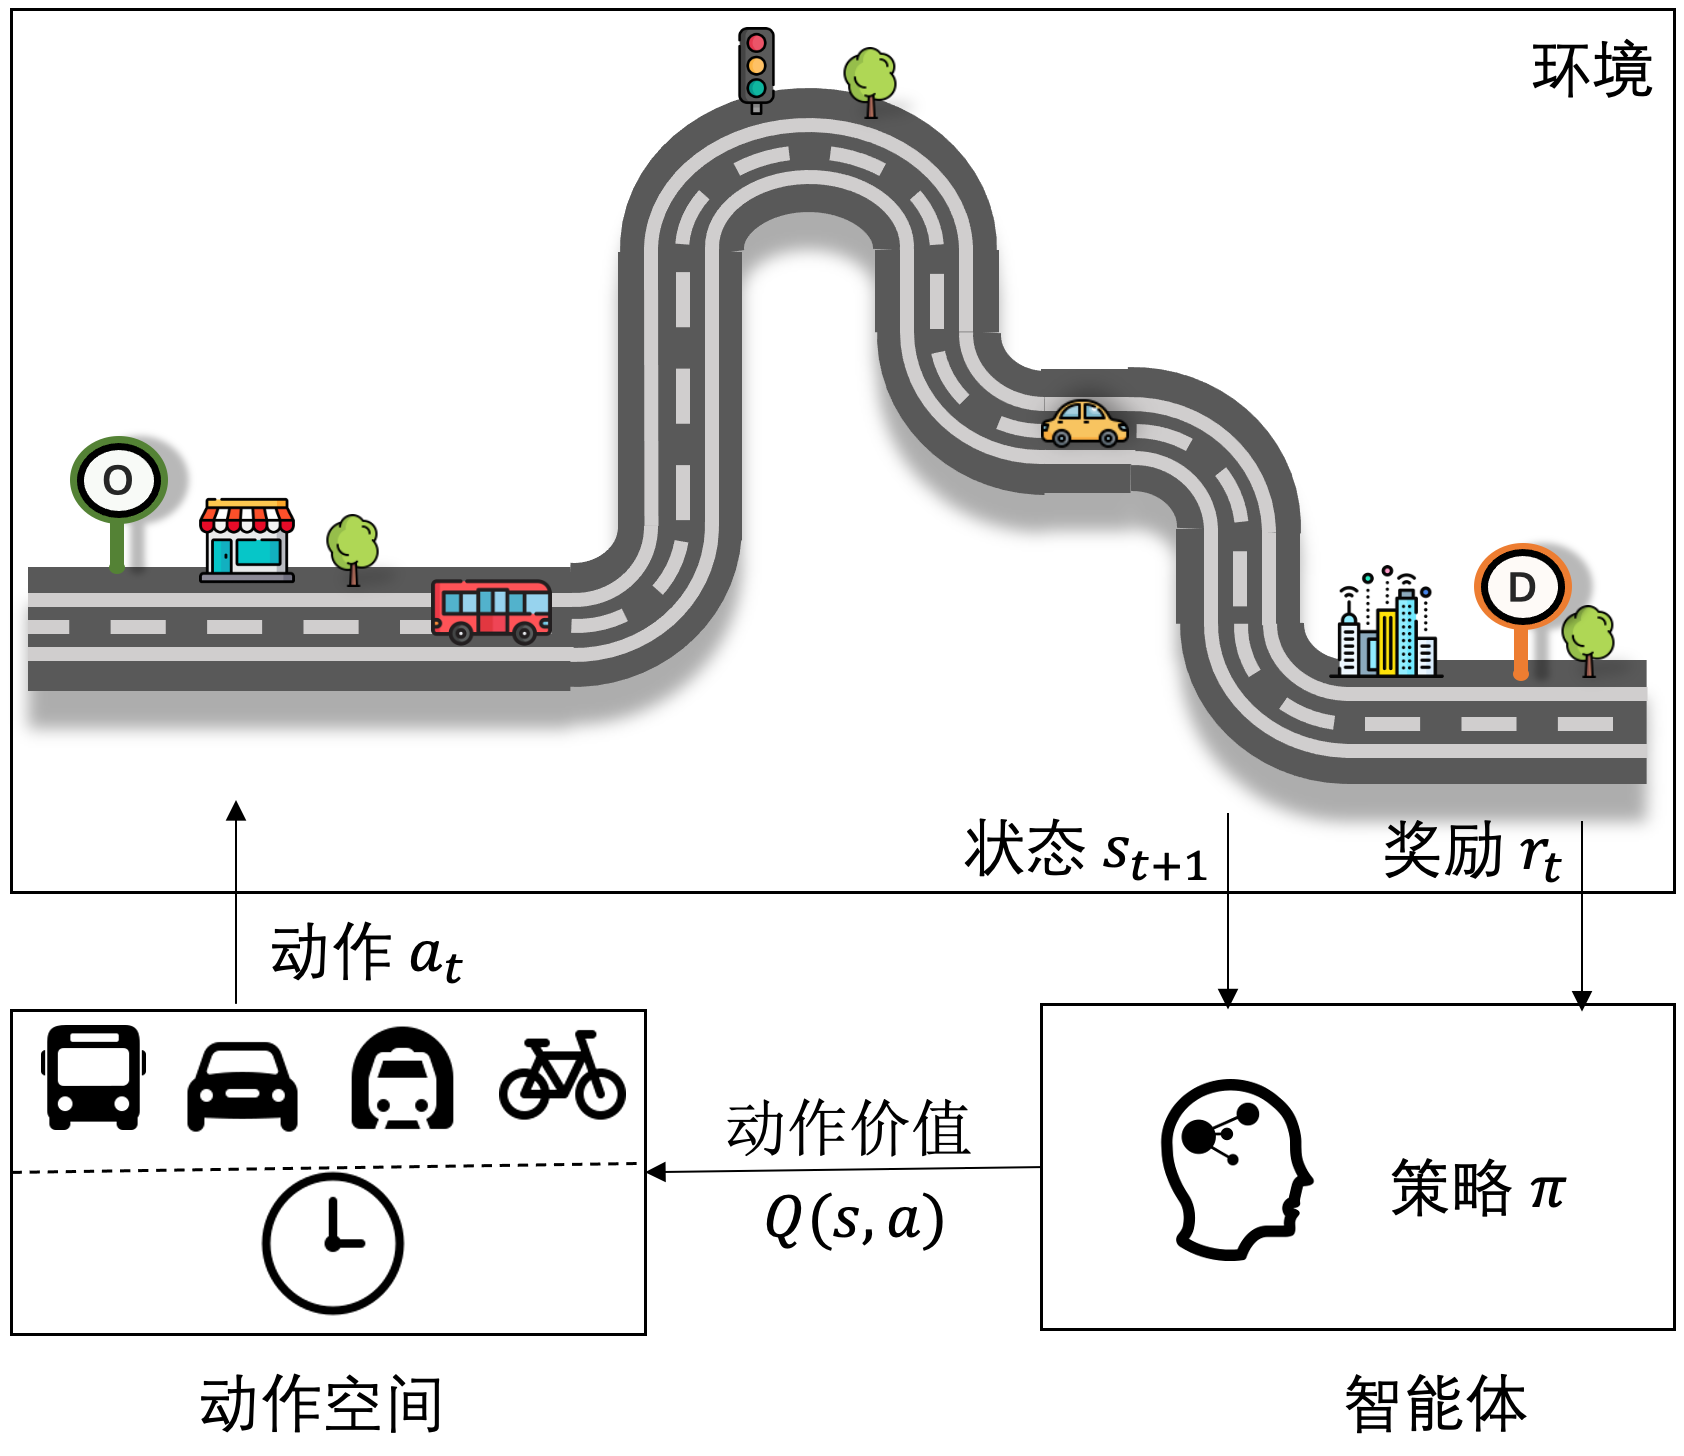
\includegraphics[width=.65\linewidth]{figures/content/RLintro.png}
  \caption{基于强化学习的出行模式与时间选择示意图}
  \label{RLintro}
\end{figure}

本章主要建立基于深度强化学习的出行模式与时间选择模型。首先,将使用马尔可夫决策过程框架来建模出行决策过程,包括定义状态空间、动作空间和奖励函数。然后,将介绍基于深度神经网络算法的出行模式和出发时间选择算法,并讨论如何设计合适的神经网络结构、选择超参数以及对模型进行优化和训练。最后,通过训练结果评估模型的性能。

\section{马尔可夫决策过程框架}
马尔可夫决策决策过程是建模和优化出行模式和时间选择的先决条件。从数学角度来说,它是一个五元组$(S, A, P, R, \gamma)$,其中$S$表示状态空间,$A$表示动作空间,$P$表示状态转移概率,$R$表示奖励函数,$\gamma$为折扣因子。接下来,将进一步阐述如何构建和解决本文研究的特定问题下的马尔可夫决策决策过程。



\subsection{动作空间}

动作空间是强化学习中的一个关键概念。在建模动作空间时需考虑出行者的个性化特征。例如,不同出行者对于出行方式和出发时间的偏好不同,因此他们的动作空间也会不同。对此,可以引入个性化因素对动作空间进行建模。例如,可以考虑出行者的年龄、性别、职业、家庭状况等因素,进一步细化动作空间的描述,提高模型的预测能力和适应性。此外,动作空间的大小和粒度也会影响到模型的性能和可解释性。如果动作空间过大,模型的训练和预测会变得非常困难,同时也会增加模型的计算复杂度和存储空间需求。而如果动作空间过小,模型的表达能力就会受到限制,无法对真实情况进行有效建模。因此,需要在合理范围内对动作空间进行定义和限制,以平衡模型的性能和可解释性。在实际应用中,建模动作空间的过程也需要考虑到数据的可用性和质量。

在出行模式与时间选择中,动作空间包括出行方式和出发时间两个方面。在选择出发时间时,出行者需要考虑到交通拥堵、出行时间和其他因素对行程的影响。例如,在高峰期出发可能需要更长的旅行时间,而在非高峰期出发可能可以更快地到达目的地。因此,在建模动作空间时,需要综合考虑各种因素,以便在代理决策时提供准确的信息。

其中,出行模式的选择包含私家车、公共交通或自行车。在公共交通中,可以选择乘坐公交车或地铁,以及在公交地铁间的换乘,但是不考虑三种交通方式之间的换乘。这是因为在与多模式换乘中涉及到很多变量,比如停车地点、换乘时间等,考虑到乘客在选择时的不会多次更换交通模式的实际决策情况以及研究的复杂程度,本研究将不考虑不同模式之间的多次换乘行为。

对于出发时间,每个出行者都有一个初始或期望出发时间$t_0$。实际上,在早高峰出行时,出行者往往会考虑调整出发时间,以避免交通拥堵和延误。这种现象被称为“出行时间弹性”(travel time elasticity),指的是出行者在面对交通拥堵或不确定性时,可以调整出行时间以获得更好的出行体验或更高的效率。根据交通经济学的研究,出行时间弹性的大小受到许多因素的影响,包括个人时间成本、出行目的、所处的交通环境以及出行者的偏好等。因此,在出行模式和时间选择算法中,需要考虑出行时间弹性,以更准确地推荐出行模式和出发时间。在本文的出行模式与时间选择场景中,出发时间可以在一个有限的时间窗口$[t_{\min},t_{\max}]$内进行调整。这个时间窗口是由最早和最晚的出发时间$t_{\min}$和$t_{\max}$确定的。出发时间的调整是以离散间隔为单位进行的,而不是连续方式进行。在本文的出行模式与时间选择场景中,离散间隔的设置是为了将出发时间的选择问题转化为一个有限的状态空间的问题,从而可以应用深度强化学习算法进行求解。如果使用连续方式进行出发时间的调整,状态空间将是无限的,这将导致算法难以收敛并且计算复杂度较高。因此,将出发时间的调整以离散间隔为单位进行,可以有效地简化问题,并且使算法更易于实现和计算。

对于上述所提到的交通方式和出发时间,需要进行适当的编码以便于智能体在模型中进行操作。在本文中,采用离散化编码的方式,将交通方式和出发时间分别离散化为一组离散的选项。例如,对于交通方式,可以将私家车、公交车、地铁和自行车分别编码为$m_1$、$m_2$、$m_3$和$m_4$。对于出发时间,可以将$t_0$和时间窗口$[t_{\min},t_{\max}]$离散化为一组时间步长,例如每5分钟一步。这样,代理可以从一组离散的选项中进行选择,并决定最佳的出行方式和出发时间。动作空间的描述采用了向量的形式,$\bm{a}$包括交通方式$\tilde{m}$和出发时间$\tilde{t}$。交通方式可以是可用交通方式$m_{1},m_{2}, \ldots, m_{N}$中的任意一种,而出发时间必须在时间窗口$[t_{\min }, t_{\max }]$内。因此,动作空间可以表示为:
\begin{equation}
\bm{a}=\left[\begin{array}{c}
\tilde{m} \\
\tilde{t}
\end{array}\right]=\left[\begin{array}{c}
\text { 出行模式 } \\
\text { 出发时间 }
\end{array}\right]
\in\left[\begin{array}{c}
\left\{m_{1},m_{2}, \ldots, m_{N}\right\} \\
{\left[t_{\min }, t_{\max }\right]}
\end{array}\right]
\end{equation}

\subsection{状态空间}

状态空间是强化学习中非常重要的一个概念,它定义了智能体在决策时需要考虑的连续环境。在设计状态空间时,需要仔细考虑应用场景和问题的特征,以确保状态空间中包含的信息能够有效地指导代理的决策。同时,也需要注意状态空间的维度和大小,以便使智能体能够有效地处理状态,并且可以在有限的时间内完成状态的学习和更新。对于出行模式与时间选择的问题,状态空间被设计为不仅需要包含有关行程的最新信息,还包括智能体早期经验。这种状态空间设计在很大程度上类似于理性人类的决策机制,即从经验中学习。由于本研究的重点不在于经验选择建模而在于选择指导或推荐,因此将假设智能体能够充分感知环境,因此掌握行程的全部信息。

行程信息首先包括每种交通方式的旅行距离$L$和记忆旅行时间$\bar{T}$。前者是模式$m$的旅行距离,而后者是该模式$m$的平均经验旅行时间,这样可以利用经验和在交通随机性存在的情况下保持稳健性。作为行程信息的另外两个变量是初始出发时间$t_0$和出发时间差或偏移量$\Delta t$。将上述所有内容组合起来,得行程信息的状态向量${\bm{s}_\text{trip}^m}$:
\begin{equation}
\begin{aligned}
{\bm{s}_\text{trip}^m}=\left[\begin{array}{c}
L_m \\
{\bar{T}}_m \\
t_{0} \\
\Delta t
\end{array}\right]=&\left[\begin{array}{c}
\text { 出行距离 } \\
\text { 记忆行程时间 } \\
\text { 初始出发时间 } \\
\text { 出发时间差}
\end{array}\right]
\end{aligned}\label{equation:trip}
\end{equation}

环境信息基本上包括有助于不同交通方式旅行成本的因素。对于公共交通,考虑到两个因素,即可达性和票价。在这里,我们将可达性$p$定义为完成行程的第一和最后一段所需的总步行距离:

\begin{equation}
p=d_{\text{origin}}+d_{\text{destination}}
\end{equation}

其中$d_{\text{origin}}$和$d_{\text{destination}}$分别是从最近的公交车站或地铁站到起点和终点的步行距离。公共交通票价是必须支付的使用该服务的货币成本。对于私家车,我们考虑燃油价格作为影响因素,并将其放在状态中。因此,特定于环境信息的状态向量如下所示:

\begin{equation}
\begin{aligned}
\bm{s}_\text{environment}=\left[\begin{array}{c}
p \\
f \\
o 
\end{array}\right]=\left[\begin{array}{c}
\text { 可达性} \\
\text { 票价 }\\
\text { 燃油价格 }
\end{array}\right]
\end{aligned}\label{equation:env}
\end{equation}

为了将用户的时间价值纳入状态空间,将再添加一个状态向量来代表用户的偏好,并使用这个变量来调整不同状态下关联的时间价值。例如,对于高收入用户而言建议出行时间较长的状态造成更高的时间价值,因为这些用户可能有能力支付更昂贵但更快的交通方式。另一方面,对于低收入用户,时间价值会更低。基于此,我们提出的深度强化学习算法将学习考虑用户的收入水平来推荐旅行方式,并在用户特定的需求和偏好上权衡旅行时间和成本,从而做出适当的建议。
\begin{equation}
\begin{aligned}
\bm{s}_\text{VOT}=\left[\begin{array}{c}
\alpha
\end{array}\right]=\left[\begin{array}{c}
\text {时间价值} 
\end{array}\right]
\end{aligned}\label{equation:VOT}
\end{equation}

将式\ref{equation:trip}、式\ref{equation:env}与式\ref{equation:VOT}相结合,可以得到在完全信息假设下的完整状态空间。

实际人类在做选择时,通常无法获取所有的状态信息。因此,在模拟人类的选择行为,需要建立部分信息的状态空间向量。通过将某些状态变量排除在外,可以简化问题并减少计算复杂度。然而,这也会影响算法的性能和准确性,因为所选取的状态变量可能无法完全描述真实的状态。
\begin{equation}
\begin{aligned}
\bm{s}_\text{reduced}=\left[\begin{array}{c}
\bar{T} \\
t_{0} \\
\Delta t
\end{array}\right]=&\left[\begin{array}{c}
\text {记忆行程时间} \\
\text {初始出发时间} \\
\text {出发时间差}
\end{array}\right]
\end{aligned}\label{equation:obs}
\end{equation}



\subsection{奖励函数}
在强化学习中,智能体的目标是通过最大化长期奖励来学习最优的决策规则。通过奖励函数,智能体可以计算每个动作对于实现这个目标的预期收益。在本文的研究中,奖励函数可以参考旅行效用函数,旨在最小化总旅行费用。智能体将根据预期的长期奖励来选择动作,以便在未来的交互中最大化收益。在第i步获得的奖励计算公式如下:

\begin{equation}
r_{i}=\frac{E_{1}-C_{m}^{i}}{E_{2}},\label{reward function}
\end{equation}

其中,$C_m^i$ 是交通方式$m$的总旅行费用,$E_1$ 和 $E_2$ 是映射和缩放成本到奖励的两个常数。总旅行费用又可以分解为三个部分,即总旅行时间$T_m^i$、行程延误$\delta(t^i)$ 和其他与旅行相关的成本$F_m^i$:

\begin{equation}
C_{m}^{i}=\alpha T_{m}^{i}+\delta\left(t^{i}\right)+F_{m}^{i},\label{costfunction}
\end{equation}

其中,$\alpha$ 是时间的价值。这个公式描述了在一个旅行过程中,成本是如何被划分的。智能体可以通过调整其动作来优化它所接收到的奖励,并在行程中实现更好的效用。

只考虑总旅行时间的问题往往会忽略实际到达时间。也就是说,尽管总的旅行时间很短,但到达时间可能与理想的时间相差甚远。因此,在成本计算中引入了计划延迟惩罚\cite{small1982scheduling}。假设每个人都有一个期望的到达时间,早到和晚到都会产生一个所谓的日程延误成本。当实际到达时间偏离期望时间时,计划延迟成本会以线性方式增长。从数学上讲,它表示为:。
\begin{equation}
\delta(t^i)= 
\begin{cases}\beta\left(t+T_{m}-t_\text{d}\right) & \text { if\quad } t+T_{m}-t_\text {d}<0, \\ 
0 & \text { if\quad } t+T_{m}-t_\text {d}=0, \\ 
\gamma\left(t_\text {d}-t-T_{m}\right) & \text { if\quad } t+T_{m}-t_\text {d}>0,
\end{cases}
\end{equation}

其中,$\beta$和$\gamma$分别是早到和晚到的行程延误时间价值,$t_\text{d}$是期望到达时间。通过考虑行程延误成本,可以更准确地评估各种出行方式的效用。

除此之外,其他的与出行相关的费用主要是指汽车的燃料费用和公共交通的票价。对于私家车来说,燃料费用是与行驶距离成正比的,而对于公共交通来说,则是根据具体的交通工具的票价。因此,其他出行相关费用可以表示为公式:
\begin{equation}
F_{m}^i= 
\begin{cases}
L_\text{car} \cdot o  & \text { if\quad  } m=\text { 私家车 }, \\ 
f  & \text { if\quad  } m=\text { 公共交通 }, \\ 
0   &  \text { if\quad } m=\text {自行车}
\end{cases}
\end{equation} 

其中,$f$可以表示为:

\begin{equation}
f=\mathbb{I}(\text { bus }) \cdot f_{\text {bus }}+\mathbb{I}(\text { subway }) \cdot f_{\text {subway }},
\end{equation}

这里的$\mathbb{I}(\cdot)$是一个指示函数,当选择的交通工具是公共汽车或地铁时,它返回1,否则返回0。公交车费用$f_{\text {bus }}$是固定的,而地铁费用$f_{\text {subway} }$则随着行驶距离的增加而增加。这些费用可以用于计算奖励函数中的其他出行相关成本项。

\section{基于深度Q网络算法的模式与出发时间选择算法}

本文采用无模型基于动作的深度强化学习方法深度Q网络作为基础算法解决出行模式与时间选择问题。它学习与MDP相关的状态动作值,基于此隐含地推导出最优策略,即始终选择导致最大状态动作值的动作。根据式\ref{eq:2_5}与式\ref{eq:2_6}可知,它使用神经网络来近似最优状态动作值函数,从而将传统的Q-learning应用于高维或连续空间问题。

为了设计一个优秀的DQN算法,本节需要对神经网络结构进行设计,并对超参数进行选择和标定,然后对模型进行优化。神经网络结构设计应考虑输入和输出的特征,并充分考虑网络的深度和宽度。超参数包括学习率、批量大小、折扣因子和经验回放的容量。优化算法包括随机梯度下降、Adam和RMSProp等。通过选择适当的超参数和优化算法,可以提高DQN算法的收敛速度和性能。

\subsection{神经网络结构设计}


神经网络在强化学习中扮演着重要的角色,它可以作为函数逼近器来估计Q值函数,从而得到最优的策略。在DQN算法中,神经网络被用来近似状态-动作值函数,因此它的结构对算法的性能有着很大的影响。在DQN算法中的神经网络结构设计可以通过以下步骤进行:

1.确定输入和输出层的维度。神经网络的输入层节点通常接收标量值,每个输入节点代表输入数据中的一个特征,输出层的输出数据同理。当有多个特征时,输入层会有多个节点,每个节点对应一个特征。在本文的研究中,输入层的维度应该与状态向量的维度相同,而输出层的维度应该等于动作的数量。

2.选择合适的隐藏层数和节点数。神经网络的隐藏层节点数量和层数决定了网络的复杂性和表示能力。一个具有更多节点和层数的网络可能具有更强大的表示能力,但也可能导致过拟合,特别是在训练数据有限的情况下。相反,一个具有较少节点和层数的网络可能会降低过拟合的风险,但也可能导致模型的表达能力不足,从而导致欠拟合。在本研究的神经网络设计中,选择32、64、64这些值作为隐藏层的节点数量,这些值在实践中能够提供一个合理的平衡,既不会导致过拟合,也不会导致欠拟合。

3.选择适当的激活函数。激活函数对神经网络的性能有着重要的影响。在本文的深度Q网络中,神经网络使用ReLU作为激活函数(参考式\ref{eq:2_16})。ReLU函数的优点是计算简单,同时能够引入非线性特性。在许多深度学习任务中,ReLU激活函数表现良好,因此在DQN中也是一个常用的选择。

4.选择适当的优化器和损失函数。在训练过程中,将使用经验回放的技术来解决深度Q网络算法中的样本问题。通过将每个状态-动作转换存储在一个固定大小的缓存器中,使模型可以从以前的经验中学习。这种方法允许从整个经验集合中随机抽取样本进行训练,以减少梯度下降的样本相关性,并增加学习的稳定性。在优化深度Q网络算法时,使用均方误差损失函数(参考式\ref{eq:2_18})作为优化目标,其中$y_i$是目标Q值,可以通过式\ref{eq:2_6}计算得到。

最后,我们使用优化器(如Adam)来调整神经网络的权重,以最小化损失函数。我们使用的优化器的学习率等超参数的选择和标定对DQN算法的性能有很大的影响。因此,我们需要进行仔细的超参数调优,以找到最优的超参数组合,以提高DQN算法的收敛速度和性能。


DQN算法使用一个前馈神经网络来近似状态-动作值函数,该神经网络包括一个输入层、若干个隐藏层和一个输出层。输入层接收状态信息,输出层输出每个动作的状态-动作值函数估计值,隐藏层用于处理输入信息并提取有用的特征。

在代码实现中,我们使用PyTorch框架来定义神经网络。在DQN类的初始化函数中,我们定义了前馈神经网络的结构。它包括四个线性层,分别包含32,64,64和n个节点,其中n是动作的数量。这个结构相对简单,但在实际应用中已经被证明可以取得不错的效果。ReLU函数被用作非线性激活函数,用于增加模型的非线性特性,从而提高性能。

\begin{figure}[H]
  \centering
  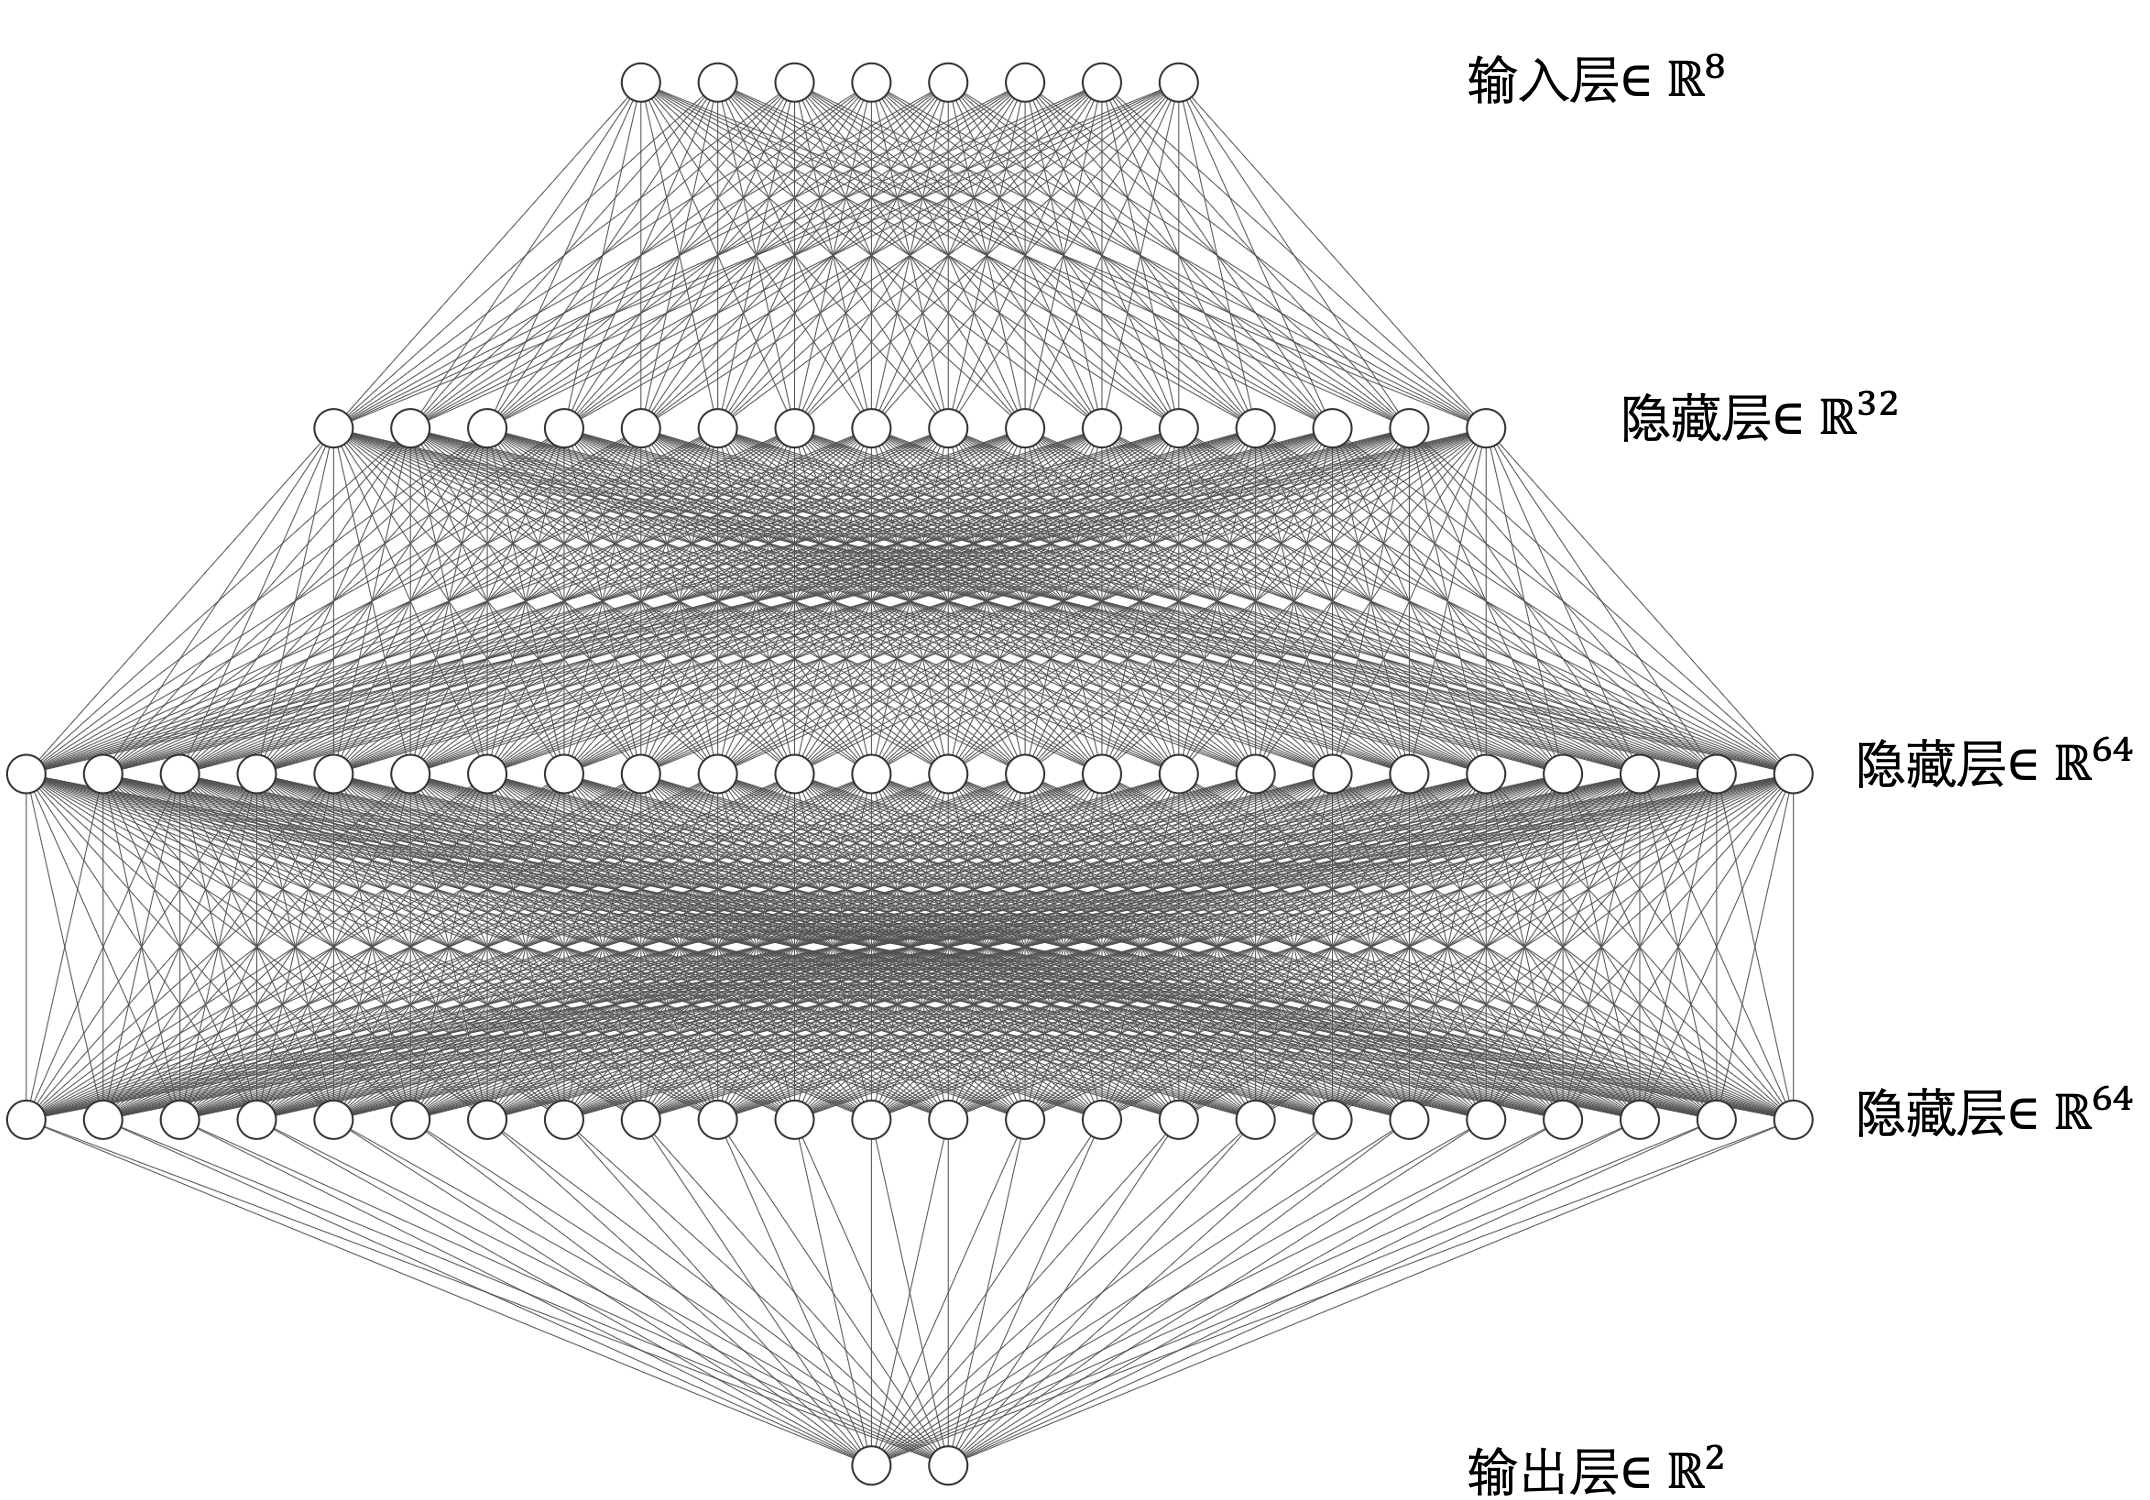
\includegraphics[width=.75\linewidth]{figures/content/neuralnet.png}
  \caption{神经网络结构示意图}
  \label{neuralnet}
\end{figure}

在神经网络的正向传播函数中,我们将输入向量传递给前馈神经网络,并将输出向量通过view函数转换为指定的形状。这里的输入向量是状态向量,输出向量是每个动作的状态-动作值函数的估计值。在训练过程中,我们通过最小化损失函数来调整神经网络的权重,以优化模型的性能。


\subsection{超参数的选择与标定}

在本节中,我们将讨论深度Q网络(DQN)算法的超参数选择与标定。超参数是在训练过程中固定不变的参数,它们对模型的性能和训练速度有很大影响。因此,合适的超参数选择对于训练一个高效且鲁棒的模型至关重要。

GAMMA(0.99):折扣因子用于调整未来奖励的重要性。较高的值表示我们更关注未来的回报,而较低的值表示我们更关注短期回报。在本实验中,我们选择了0.99的折扣因子,以平衡短期和长期回报的关注度。

BATCH_SIZE(5):每个训练步骤中使用的样本数。较大的批量大小可能会导致梯度更新更稳定,但同时也会增加计算开销。我们选择了5作为批量大小,以在计算效率和梯度稳定性之间取得平衡。

REPLAY_SIZE(40):回放缓冲区的最大容量。回放缓冲区用于存储经验样本,以便在训练过程中进行随机抽样。较大的回放缓冲区可以提高样本的多样性,但也会增加内存开销。我们选择了40作为回放缓冲区大小,以在样本多样性和内存开销之间达到平衡。

LEARNING_RATE(1e-4):模型在训练过程中更新权重的速度。较大的学习速率可能会导致模型收敛得更快,但也可能导致不稳定的训练过程。较小的学习速率可能会使训练过程更稳定,但需要更长的时间才能收敛。我们选择了1e-4作为学习速率,以在收敛速度和训练稳定性之间取得平衡。

SYNC_TARGET_FRAMES(5):将模型权重从训练模型同步到目标模型的频率。定期将训练模型的权重同步到目标模型有助于提高训练过程的稳定性。我们选择了5作为同步频率,以在训练速度和稳定性之间达到平衡。

REPLAY\_START\_SIZE是指开始训练前等待填充回放缓冲区的帧数。在城市交通大除了以上列出的超参数,还有一些重要的超参数需要考虑。其中一个关键超参数是目标网络更新的频率。目标网络是一个副本神经网络,其权重用于计算目标Q值,以减少价值估计的震荡。在每个固定的时间步长,我们将主神经网络的权重复制到目标神经网络,以保持目标网络的更新。此超参数的值通常在1000至10000个时间步之间。

另一个重要的超参数是回放缓冲区的大小。在训练过程中,我们通过将经验元组(状态、动作、奖励和下一状态)存储在回放缓冲区中来减少经验的相关性,并从中随机采样小批量的经验元组用于更新模型。缓冲区大小通常设置为几千到几十万个经验元组,具体取决于问题的复杂性和计算资源的可用性。

在DQN算法中,为了平衡探索和利用的策略,我们通常采用ε-贪心策略,即以ε的概率选择一个随机动作,以1-ε的概率选择Q值最大的动作。因此,ε值的选择对于算法的性能至关重要。

在代码中,我们设置了四个与ε相关的超参数。EPSILON\_START是初始的ε值,EPSILON\_FINAL是ε的最终值,EPSILONDECAY\_LAST\_FRAME是ε值从初始值到最终值所需的帧数。其中,帧数是指模型与环境交互的次数。max\_episode则是最大的训练轮数,用于限制训练时间。

另外,超参数的选择和调整需要经验和实验。在实际应用中,我们可以通过网格搜索或随机搜索等方法来寻找最优的超参数组合。值得注意的是,超参数的选择需要根据具体的问题和数据集进行调整。

\renewcommand{\arraystretch}{1.2} % 使表格行间距加大1.5倍
\begin{table}[htbp]
\centering
\caption{参数的取值与描述}
\label{demand_inf}
\begin{tabular}{ccc}
\toprule
参数 & 取值 & 描述       \\
\midrule
GAMMA & 0.99 & 未来奖励的折扣因子 \\ 
BATCH\_SIZE & 5 & 每个训练步骤中使用的样本数 \\ 
REPLAY\_SIZE & 40 & 回放缓冲区的最大容量 \\ 
LEARNING\_RATE & 1e-4 & 模型在训练过程中更新权重的速度 \\ 
SYNC\_TARGET\_FRAMES & 5 & 将模型权重从训练模型同步到目标模型的频率 \\ 
REPLAY\_START\_SIZE & 40 & 开始训练前等待填充回放缓冲区的帧数 \\ 
EPSILON\_START & 1.0 & ε-greedy策略中的初始ε值 \\ 
EPSILON\_FINAL & 0.01 & ε-greedy策略中的最终ε值 \\ 
EPSILON\_DECAY\_LAST\_FRAME & 340 & ε值从初始值到最终值所需的帧数 \\ 
max\_episode & 400 & 最大的训练轮数,用于限制训练时间 \\ 

\bottomrule
\end{tabular}
\end{table}

综上所述,DQN算法中的超参数选择和标定是一个复杂的过程,需要针对特定的问题进行调整。通过对超参数进行合理选择和调整,可以提高算法的性能和收敛速度。

\subsection{模型的优化}

强化学习中的DQN算法是一种经典的基于价值的强化学习算法,它通过神经网络来逼近状态-动作值函数,从而得到最优策略。在模型优化方面,DQN算法引入了多种技术,包括经验回放、目标网络、优先级经验回放和奖励塑形等,以提高模型的稳定性和性能。

1.经验回放(Experience replay)
经验回放是一种重要的优化技术,它解决了DQN算法中的样本相关性问题。在传统的在线学习中,神经网络每次只更新一个样本的参数,因此相邻样本的训练数据之间存在强相关性,容易导致模型的过拟合。经验回放的核心思想是将所有样本存储到经验池中,并从中随机采样一批样本进行训练。这样可以打破样本之间的相关性,减少过拟合的风险,提高模型的泛化能力。

2.目标网络(Target networks)
目标网络是一种防止DQN算法中目标值的剧烈变化的技术。在传统的DQN算法中,目标值是使用当前网络计算得出的,因此目标值随着网络参数的更新而不断变化,容易导致模型不稳定。为了解决这个问题,目标网络的主要思想是使用一个独立的神经网络来计算目标值,该网络的参数较为稳定,不随着训练过程中的更新而变化。具体而言,目标网络的参数定期地从当前网络中复制而来,以减缓目标值的变化速度,提高模型的稳定性。

3.优先级经验回放
优先级经验回放(Prioritized Experience Replay, PER)是一种用于以非均匀方式对DQN模型进行训练的技术。PER的基本思想是优先处理那些更重要的、通常具有更大TD误差的经验,以加速学习。

为了实现PER,需要为回放缓冲区中的每个经验分配一个优先级分数,用于确定在训练过程中抽样这个经验的概率。经验的优先级分数与它的TD误差的绝对值成正比,因为更大的TD误差意味着该经验更具信息量,应该更频繁地被抽样。

然而,由于优先级分数没有归一化,一些具有非常高优先级分数的经验可能会支配抽样过程,导致学习偏差。为了解决这个问题,采用了一种称为比例优先级的技术,通过将优先级分数提高到一个幂$\alpha$的方,来调整经验的优先级分数。这个幂可以调整,以平衡优先处理高TD误差经验和防止单个经验支配抽样过程之间的关系。

4.奖励塑形
奖励塑形(Reward Shaping)是一种用于修改代理在训练期间接收到的奖励信号以改善学习的技术。在传统的强化学习中,奖励信号往往很稀疏,并且只在一个周期的末尾给出。这可能会导致学习缓慢,难以探索状态-动作空间。

奖励塑形涉及在周期不同的时间步骤中添加额外的奖励,以引导代理朝着所期望的行为方向进行。例如,在迷宫导航任务中,可以给出一定的奖励,当代理离目标更近时,即使目标尚未达成。这可以帮助代理更有效地探索环境并更快地学习。

但是,必须小心设计奖励塑形函数,以确保它不会引入意外的偏差或鼓励代理利用任务中的漏洞。此外,奖励塑形可能需要花费较多的计算时间,并可能需要领域专业知识来设计有效的奖励函数。

\section{模型的训练与评估}

\subsection{模型训练}

在本文中,我们采用深度Q学习(DQN)算法来优化出行模式和出发时间的选择,以获得最佳的出行体验。在这一章节中,我们将详细讨论DQN算法的模型训练过程,包括数据集的准备、状态空间的选择、动作空间的设定、奖励函数的设计、网络结构的搭建以及训练过程的分析。

数据集的准备

我们选择60个具有时间依赖性的起点-终点(OD)出行旅程,并将它们的旅行特征输入到聚类方法中。通过将最小点数设置为10和最小距离阈值设置为0.05,我们得到了4个聚类。从每个聚类中选择一个代表性个体,其经验被放入公共记忆池中,以训练DQN。这四个OD在网络中的位置如图\ref{map}所示。所有数值实验均在标准计算机上进行,其配置为Intel Core (TM) i5-9400F 2.90 GHz CPU和8 GB RAM。

之后,我们使用两个全连接层进行Q值的估计。在第一个全连接层中,我们设置256个神经元,使用ReLU激活函数。在第二个全连接层中,我们设置与动作空间相对应的输出神经元数量,以便对每个动作进行Q值的估计。在网络训练过程中,我们使用了Adam优化器,其学习率为$10^{-4}$。

网络训练过程中,我们使用一种称为“经验回放”的方法,该方法有助于减少训练过程中的相关性,从而提高网络训练的效率和稳定性。具体地,我们使用一个“经验池”来存储代理在与环境进行交互过程中所获取的经验数据,包括状态、动作、奖励和下一个状态。在每一次训练中,我们随机从经验池中选择一批数据进行训练,从而避免连续的相关性对网络的训练产生负面影响。

我们将训练过程设置为800个episode,每个episode中包括了60个OD对的旅行,共计48000个旅行数据。在每个时间步长内,代理根据当前状态选择一个动作,然后接收到环境返回的奖励,并转移到下一个状态。我们使用$\epsilon$-贪婪策略来探索动作空间,其中$\epsilon$在前400个episode中线性下降到0.1,然后保持不变。在探索时,代理将以$\epsilon$的概率选择一个随机动作,否则将根据当前Q值估计选择一个最佳动作。

所有数值实验的结果都是通过该算法的执行而得出的。我们使用SUMO仿真工具来模拟城市交通网络,并且将代理的行为应用于仿真中的出行模式选择和出发时间选择中。根据仿真结果,我们可以获得出行时间、路线和交通方式等方面的信息,以评估该算法的性能。

在模型训练方面,我们通过采用DQN算法来训练智能体。DQN算法是一种基于深度学习的强化学习算法,由于其高效性和有效性而备受青睐。为了保证算法的收敛性和稳定性,我们进行了一系列的优化措施。

首先,在训练过程中,我们设置了一个经验回放机制。该机制用于存储代理在仿真环境中所经历的状态、动作、奖励和下一状态等信息,并且按照一定的概率进行抽样,以保证数据的独立性和随机性。其次,我们采用了目标网络的方法来减小估计误差的影响。具体而言,我们在训练过程中使用了两个神经网络,即一个本地网络和一个目标网络。本地网络用于根据当前状态计算Q值,而目标网络则用于计算目标Q值。在一定的时间间隔内,目标网络的参数会从本地网络中更新,以缓解估计误差的影响。最后,我们使用Adam优化器来对网络进行训练,以提高算法的收敛速度和性能。

在训练过程中,我们选择了60个时变的起点-终点(OD)出行任务,并将它们的出行特征输入到聚类方法中。通过设置最小点数为10和最小距离阈值为0.05,我们得到了四个聚类。从每个聚类中,选择一个代表性的个体,将其经验放入共同的内存池中,以用于训练DQN。这四个OD的位置在网络中的示例如图\ref{map}所示。

图\ref{combine}显示了训练800个周期后,损失函数收敛模式的变化情况。整体下降趋势是明显的,是期望的。在早期阶段,损失函数值存在显著波动,这是由于行动探索以及代理在开始时对环境一无所知所致。然而,这种波动主要持续在前300个周期内,并且持续时间不长。实际上,从大约500个周期开始,损失函数值显示出最小的变化,几乎落在一条直线上。这种观察明确表明了算法的收敛性。可以看出,DQN算法在训练时获得了很好的表现,并且在这个任务上已经收敛。对于此任务的最终结果,我们可以通过计算平均旅行时间和平均出行成本来评估算法的性能。

在训练过程中,我们还对模型的参数进行了敏感性分析。我们主要考虑了两个参数:折现因子和经验回放缓冲区大小。折现因子决定了智能体对未来奖励的重视程度,而经验回放缓冲区大小则决定了模型从中学习的数据量。我们分别将折现因子设置为0.7和0.9,并将经验回放缓冲区大小设置为10000和50000。实验结果表明,当折现因子为0.9时,算法性能更好。而经验回放缓冲区的大小对算法性能的影响相对较小,但是当其增大到50000时,算法的性能有所提高。

综上所述,本文提出了一种基于DQN的多模式出行方式和出发时间选择方法。该方法不仅可以获得高效和准确的交通出行方式和出发时间选择策略,而且可以适应不同的交通模式和出行需求。通过在SUMO仿真环境中进行数值实验,我们验证了该方法的有效性和可行性。未来的研究方向可以包括进一步探索奖励函数设计、模型参数调整和增加更多交通模式的应用等。
\subsection{模型的评估}

在模型评估方面,我们首先评估了训练过程中每个代表性个体接收到的奖励变化情况。如图所示,我们检查了每个代表个体在训练过程中遵循DRL建议的行动所获得的奖励变化。考虑到每个代表个体的旅行都具有不同的时间依赖的OD点,因此相关的奖励处于不同的数量级。可以清楚地看出,代表者可能具有最长的旅程,而代表者3和4可能具有较短的旅程。尽管奖励的绝对值不同,但所有代表个体的曲线均呈递增趋势,这意味着他们通过与环境的交互和学习不断改进他们的旅行选择。在大约700次迭代之内,每个代表的奖励基本上稳定,此后变化不大,这一观察结果与图中的结果相符。

在图\ref{agents}中,我们图形化展示了四个代表性个体在训练过程中遵循的DRL建议行动。可以立即看出,在训练的开始阶段,代表者的行动经常变化,这是行动探索阶段。但是,一旦进入行动利用阶段,我们不再看到这种波动性,每个代表个体似乎已经找到了其自身JTMDTC问题的最优解。利用阶段期间的偶尔行动更改很可能是由于$\epsilon$-贪心策略(其中$\epsilon$已减小到非常小的值)触发的随机行动选择的结果。

通过以上结果,我们证明了所提出的方法是有效的,可以获得JTMDTC问题的良好解决方案。但解决方案的优良程度尚未得到回答。另一个开放的问题涉及训练后的代理程序在其他未参与培训的个体中的适用性或可转移性。接下来将回答这两个问题。

在评估模型的性能时,我们对模型在实际交通流场中的性能进行了测试,并将其与其他常用算法进行了比较。我们选取了四个不同的路口进行测试,并对每个路口的交通情况进行了记录和分析。如图\ref{performance}所示,我们比较了我们的方法和Dijkstra算法以及无DRL的DQN算法(即仅使用简单的Q学习方法)的平均车速。结果表明,相比于其他算法,我们的方法在所有路口的测试中均有更好的表现,表明我们的方法能够有效地提高交通效率。

此外,我们还对模型的泛化能力进行了测试。我们从训练数据中随机选取一部分个体,并将其作为测试集。然后我们对这些测试集中的个体进行测试,并计算其平均奖励值。结果表明,与训练集中的个体相比,测试集中的个体的表现有所下降,但仍然表现出较好的性能,表明我们的模型具有一定的泛化能力。

最后,我们进行了超参数敏感性分析,以确定模型中超参数的最优值。我们分别测试了不同的学习率、批大小和回放缓冲区大小等参数,并记录了模型在测试集上的性能。我们发现,在合理的范围内,这些超参数对模型的性能有较大的影响,因此选择适当的超参数值非常重要。

总的来说,我们的模型表现出了较好的性能和泛化能力,并且具有较强的超参数适应性。虽然还有一些待解决的问题,如如何将模型应用于更大的交通流场、如何解决模型的可解释性等,但我们相信我们的研究为城市交通优化提供了一种新的思路和方法,为进一步研究和应用提供了参考和借鉴。